\documentclass[a4paper,12pt, twoside]{book} % nie: report! book
%\documentclass[a4paper,12pt,twoside,openany]{report}

% pakiety
\usepackage{polski} % lepiej to zamiast babel!
\usepackage[utf8]{inputenc} % w razie kłopotów spróbować: \usepackage[utf8x]{inputenc}
\usepackage{fancyhdr} % nagłówki i stopki
\usepackage{indentfirst} % WAŻNE, MA BYĆ!
\usepackage[pdftex]{graphicx} % to do wstawiania rysunków
\usepackage{amsmath} % to do dodatkowych symboli, przydatne
\usepackage{graphicx}
\usepackage[pdftex,
            left=3.5cm,right=2.5cm,
            top=1in,bottom=1in]{geometry} % marginsy
%\usepackage[inner=3.5cm,outer=2.5cm]{geometry}left=1in,right=1in,
\usepackage{amssymb} % to też do dodatkowych symboli, też przydatne
\usepackage{pdfpages} % żeby wstawić stronę tytułową
\graphicspath{ {./img/} }
\usepackage{booktabs,siunitx,array,threeparttable}
\sisetup{group-minimum-digits=4}
% jesli potrzeb, można oczywiście wstawić inne pakiety i swoje definicje...
\usepackage[backend=bibtex, sorting=none]{biblatex}
\usepackage{listings}
\addbibresource{references.bib}


% definicje nagłówków i stopek
\pagestyle{fancy}
\renewcommand{\chaptermark}[1]{\markboth{#1}{}}
\renewcommand{\sectionmark}[1]{\markright{\thesection\ #1}}
\fancyhf{}
\fancyhead[LE,RO]{\footnotesize\bfseries\thepage}
\fancyhead[LO]{\footnotesize\rightmark}
\fancyhead[RE]{\footnotesize\leftmark}
\renewcommand{\headrulewidth}{0.5pt}
\renewcommand{\footrulewidth}{0pt}
\addtolength{\headheight}{1.5pt}
\fancypagestyle{plain}{\fancyhead{}\cfoot{\footnotesize\bfseries\thepage}\renewcommand{\headrulewidth}{0pt}}


% interlinia
\linespread{1.25}


% treść
\begin{document}
\sloppy



\thispagestyle{empty}


\includepdf{stronatytulowa}
% najpierw uzupełnij w 'stronatytulowa.odt' openoffice i wyeksportuj do 'stronatytulowa.pdf'

\newpage{}

\thispagestyle{empty}

\newpage{}



\tableofcontents{}

\chapter*{Wstęp} % z gwiazdką, więc bez numerka...
\addcontentsline{toc}{chapter}{Wstęp} % ...ale w spisie treści ma być
Stale rozrastające się zasoby wiedzy, katalogowanie jej, uporządkowanie dla systemów informatycznych na całym świecie w sposób zrozumiały, oraz pozwalający na łatwe przeszukiwanie i wykorzystanie, tak dużych ilości informacji powodowało wiele problemów w ostatnich dekadach. W roku 2018, ilość danych w internecie wynosiła 10 jottabajtów (10 000 000 000 000 000 GB) \cite{EwelinaStoj.}, stale zwiększając swój rozmiar po dziś dzień. Naturalną kwestią jest to, że wiele ważnych informacji jest pomijane, zapisane w sposób nieintuicyjny lub niezrozumiały, dla ludzi i maszyn. Ontologie, oraz języki jakimi są zapisywane, takie jak np. Web Ontology Language (OWL) \cite{wow}, rozwiązują problem standaryzacji danych w celu zwiększenia ich użyteczności.

\chapter*{Cel i zakres}
Celem pracy jest przybliżenie tematyki ontologii (w tym języków opisu ontologii a także metodologii
i metodyk wytwarzania), oraz wykonanie analizy i projektu systemu tworzenia/zarządzania ontologiami (Ontology development environment - ODE).
Została wykonana analiza jednego z najpopularniejszych programów do edycji ontologii - Protégé. Przeprowadzenie ankiety, oraz podsumowanie jej wyników, pozwoliło wyciągnąć wnioski, jak duża jest grupa docelowa, oraz jakie problemy napotkali w przeszłości ankietowani, korzystający z takiego oprogramowania. Zostały zebrane wymagania, stworzone diagramy klas, i przypadków użycia, oraz został przedstawiony interfejs graficzny. Implementacja wcześniej zaprojektowanych klas, oraz wersja demonstracyjna przedstawiająca wygląd oprogramowania, potwierdziła użyteczność zaproponowanych funkcji, oraz estetykę.

\chapter{Ontologia}
Ontologia ma wiele różnych definicji. Jak podaje PWN, słowo ontologia pochodzi od greckich słów óntos, czyli byt, oraz lógos, czyli nauka. Początkowo ontologia była działem filozofii zajmującym się badaniem czym jest byt \cite{PWN}. Aktualnie w informatyce ontologia, często definiowana jest jako formalna reprezentacja dziedziny wiedzy \cite{wikipediaont}, która opisuje obiekty(byty) wraz z łączącymi je relacjami. 
Ontologie mogą różnić się ze względu na materiał, czy zakres.
Wyróżniamy \cite{Strozewski.2004}:
\begin{itemize}
	\item wysokiego poziomu(z ang. top-level lub upper ontology) zajmujące się pojęciami szerokimi, które można dopasować do każdej dziedziny \cite{wikipediaupper}
	\item dziedzinowe, zajmujące się opisem bytu w konkretnej dziedzinie
\end{itemize}

Ontologie, są używane w semantycznych wyszukiwarkach np. filmów \cite{6508326}. Słowa, które wpisywane są do takiej wyszukiwarki muszą zostać przeanalizowane w celu pokazania użytkownikowi treści, które są najbardziej zbliżone do złożonego zapytania. Wyszukiwarka analizując tekst szuka relacji między danymi wyrazami, przez co może podać dokładniejszy wynik, niż gdyby nie zwracała uwagi na związki między nimi. 

Ontologie są również stosowane w medycynie, gdzie dane biomedyczne są zmieniane w praktyczne wskazówki, które pomagają podejmować ważne decyzje \cite{protegeabout}.

Do tworzenia i zarządzania nimi stosuje się edytory ontologii, które zostały opisane w następnym rozdziale.
\section{Języki}
\subsection{Języki związane z ontologiami}
Jednym z pierwszych języków do zapisu ontologii był Knowledge Interchange Format (KIF) \cite{wikipediaont}, który powstał w latach 90. XX wieku. Jak sama nazwa wskazuje był formatem, który służył do wymiany wiedzy między np. różnymi programami. Mógł być wykorzystywany do takich szerokich pojęć jak np. to, że każda istniejąca osoba ma matkę (Rys. 1.1). Oparty jest na logice "first order", czyli na węższym rachunku predykatów. Kwantyfikator/predykat może wyrazić wiedzę na temat konkretnej domeny np. jeśli coś jest krajem, to zajmuje jakąś powierzchnię. W zdaniu "Kacper powiedział, że wszystko co ma powierzchnię jest państwem" predykat "powiedział" łączy zdanie z obiektem Kacper. Złożoność obliczeniowa zwiększa się wraz ze wzrostem skomplikowania.

\begin{figure}[h]
	\centering
	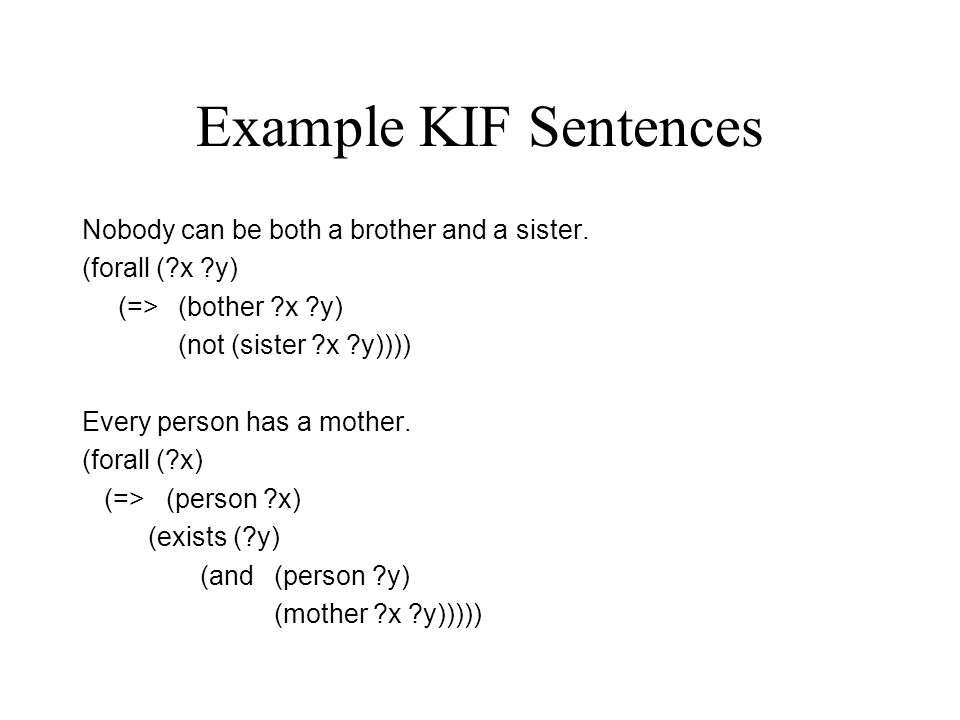
\includegraphics[scale=0.35]{slide_9.jpg}
	\caption{Przykład użycia KIF (źródło: \cite{KIF})}
\end{figure}

Kolejnym znanym językiem jest Loom. Ostatnia stabilna wersja oznaczona numerem 4.0 została wypuszczona w 1999 roku. Język ten został stworzony przez grupę badawczą z Uniwersytetu Południowej Kalifornii \cite{wikipedloom}. Loom w przeciwieństwie do KIF jest językiem opartym na logice opisowej tzn. takiej, która jest o wiele łatwiejsza do zrozumienia przez człowieka, nie odstrasza złożonością i syntaktyką, oraz łatwo ją wdrożyć na dużą skalę. Jest segmentem logiki pierwszego rzędy ze zmianami i ograniczeniami. 

\subsection{OWL}
Kolejnym bardzo popularnym językiem do zapisu ontologii jest Web Ontology Language (OWL).
\begin{figure}[h]
	\centering
	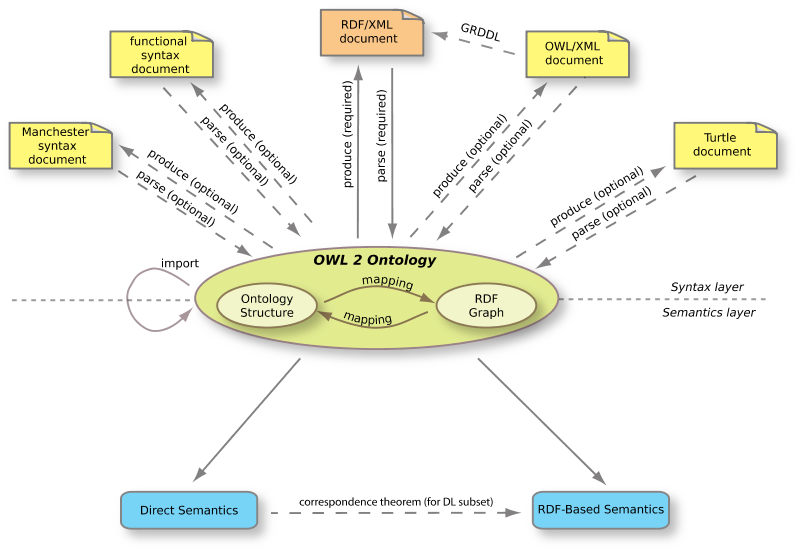
\includegraphics[scale=0.65]{OWL2-structure2-800.png}
	\caption{Struktura OWL2 (źródło: \cite{owldok})}
\end{figure}
 OWL został stworzony do reprezentowania bardzo dużych zbiorów wiedzy na wiele tematów \cite{wow}. Jego pierwszą oficjalną wersję wydano w 2004 roku, a następnie w 2009 premierę miała jego kolejna duża edycja, którą była OWL2 \cite{C.MariaKeet.2020}.
 Wydanie OWL2 przyczyniło się do wzrostu zainteresowania tym językiem co skutkowało, wzrostem ilości narzędzi dla developerów, oraz zaczęto częściej wprowadzać ontologie do systemów informatycznych. Jednym z najbardziej popularnych języków używanych z ontologiami jest OWL2.
 
 
 Resource Description Framework(RDF) \cite{wow}, który pierwszy raz został upubliczniony 28.02.1996 i którego ostatnia aktualna wersja została wydana 25.02.2014 jest językiem zaprojektowanym jako model abstrakcyjny, który standaryzuje jak dane są połączone ze sobą \cite{wikipediaRDF}. RDF jest złożony z trójek (Rys. 1.3):
\begin{itemize}
	\item podmiot
	\item predykat
	\item obiekt/przedmiot
\end{itemize}
\begin{figure}[h]
	\centering
	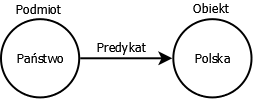
\includegraphics[scale=0.75]{Diagram1.png}
	\caption{Trójka RDF}
\end{figure}

Manchaster syntax jest składnią stworzoną, w taki sposób, aby ludziom było łatwiej ją rozumieć np. po przez zamianę znaku $\vee$ na \textbf{\textit{or}} lub $\neg$ na \textbf{\textit{not}}, które ułatwia czytanie osobom niezaznajomionym z logiką opisywaną za pomocą symboli \cite{C.MariaKeet.2020}. %78str

Nałożone przez XML standardy, które uniemożliwiły kodowanie niektórych grafów RDF \cite{turt} (niektóre predykaty Uniform Resource Identifier(URI) \cite{uri} zostały zabronione, oraz zakazane zostało kodowanie niektórych punktów kodowych (Unicode codepoint)), wymusiły stostowanie innego języka jakim jest \textbf{\textit{turtle}}, a który nie posiada tych ograniczeń \cite{turt}.
O ile, jak sama nazwa wskazuje, RDF-based semantic (Rys. 1.2) bazuje na semantyce RDF, tak semantyka bezpośrednia (Direct Semantic) jest własną semantyką OWL, którą można przetransferować do semantyki bazującej na RDF. 

\section{Metodologie i metodyki}
W określeniu, czy stworzona przez nas ontologia jest poprawna pomocne są metodyki i metodologie.
Metodologie można podzielić na:
\begin{itemize}
	\item wysokiego poziomu(macro-level), które są ogólne, mówiące o procesie
	\item mikro poziomu(micro-level), skupiające się na tworzeniu ontologii
\end{itemize}
\subsection{Metodologie wysokiego poziomu}
Metodologie są zbiorem pewnych zasad, którymi należy się kierować, aby osiągnąć jakieś zamierzone cele.
Metodologie wysokiego poziomu(macro level) pozwalają projektować ontologie w sposób ustrukturyzowany. Głównymi krokami są:
\begin{itemize}
	\item specyfikacja - kto będzie korzystał, w jaki sposób, zastosowania
	\item konceptualizacja - analiza ryzyka(np. finansowego), analiza problemu, przygotowanie dokumentu koncepcyjnego \cite{kon}
	\item formalizacja - zamiana modelu konceptualnego na formalny
	\item implementacja - wdrożenie projektu (np. stworzenie ontologii)
	\item obsługa - poprawki, aktualizacje
\end{itemize}
Natomiast istnieje wiele innych kroków, które nie zostały wymienione w tych punktach, a warto o nich wspomnieć. Takimi są np. tworzenie dokumentacji, czy system kontroli wersji. Przez to, że powstawanie ontologii to bardzo złożony proces, może on różnić się ze względu na złożoność problemu, inne podejście lub różne domeny.
Z czasem, rozwój ontologii wymuszał coraz to nowsze podejścia do projektowania ich, czego skutkiem jest metodologia NeON \cite{C.MariaKeet.2020}. Zamiast 5 kroków wymienionych wyżej, zaczęto stosować bardziej indywidualne ścieżki tworzenia ontologii (Rys. 1.4) oraz rozwinięto pytania kompetencyjne(CQ - Competency Questions).
\begin{figure}[h]
	\centering
	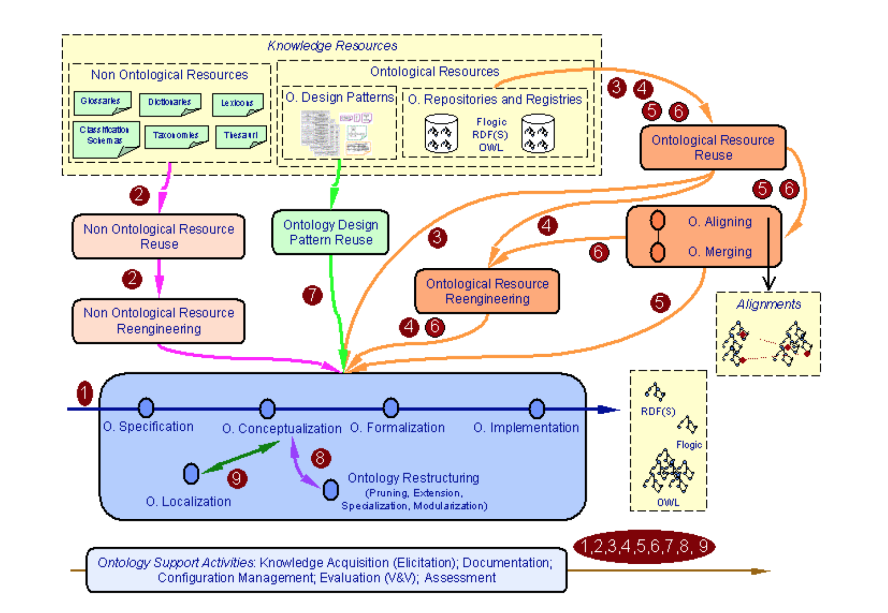
\includegraphics[scale=0.75]{NeON.png}
	\caption{Tworzenie ontologii (źródło: \cite{NeON})}
\end{figure}
CQ są to pytania na które ontologia konkretnej domeny powinna odpowiedzieć. Dla przykładu można podać pytanie "Które rzeki płyną do morza" dla ontologii mówiącej o państwie.
\begin{figure}[h]
	\centering
	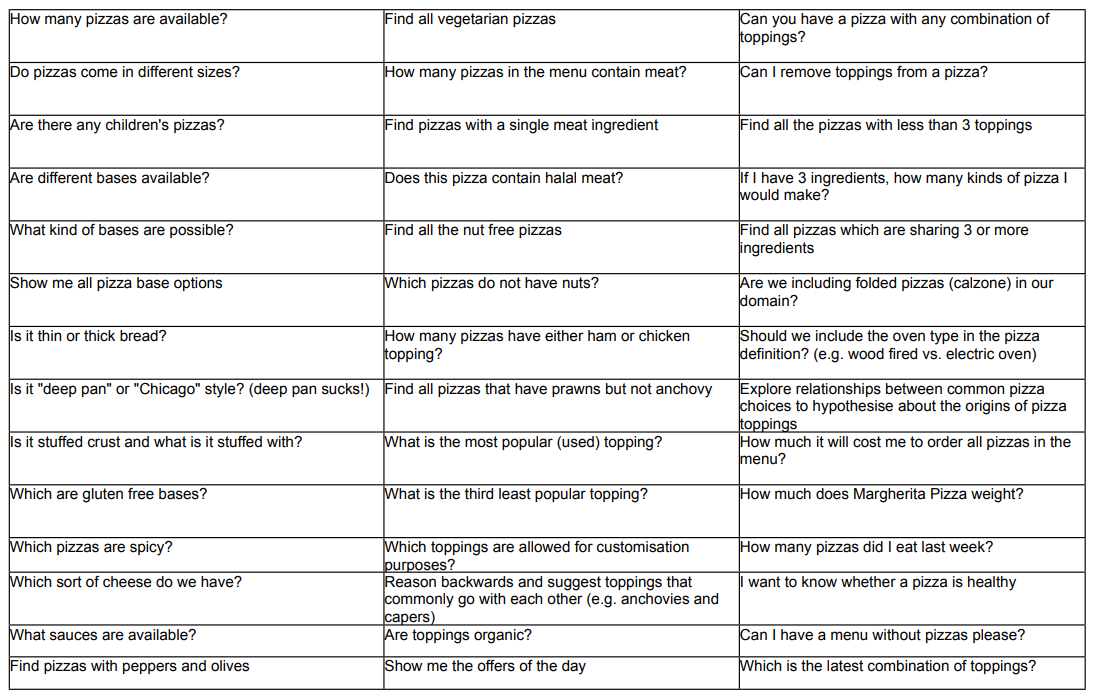
\includegraphics[scale=0.55]{CQ.png}
	\caption{Przykłady pytań koncepcyjnych (źródło: \cite{CQ})}
\end{figure}

Kolejną metodologią jest metodologia koła życia(z ang. lifecycle) \cite{C.MariaKeet.2020}(Rys. 1.6), w której przechodzenie z jednej fazy do drugiej następuje płynnie. Można przedstawić ją formie koła, które jest podzielone na część projektowania(strona prawa, czerwona), oraz na część użytkową(strona lewa, niebieska).
Wyróżniamy tam takie fazy jak:
\begin{itemize}
	\item opracowanie wymagań
	\item analiza ontologiczna
	\item projektowanie ontologii
	\item projektowanie systemu
	\item rozwój i ponowne wykorzystanie ontologii
	\item rozwój i integracja systemu
	\item zastosowanie
	\item obsługa i konserwacja
\end{itemize}
\begin{figure}[h]
	\centering
	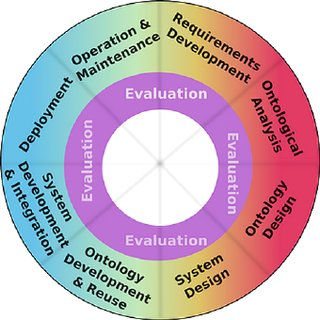
\includegraphics[scale=0.85]{lifecycle.jpg}
	\caption{Metodologia koła życia (źródło: \cite{lifecycle})}
\end{figure}

 Metodologia dotycząca zarządzania projektami nazywana Agile \cite{agile}, pomaga po przez samo organizujące się zespoły, zwiększyć komunikacje w grupie za sprawą częstszych spotkań, oraz zredukować stres, ponieważ zespoły same decydują o terminach realizacji zadań, które narzucane, często są nierealne do zrealizowania. W tym podejściu ważniejsze jest współdziałanie, oraz dostarczenie działającego produktu, niż rozbudowana dokumentacja, lub trzymanie się sztywno ram projektu.

\subsection{Metodologie mikro poziomu}
Metodologie mikro poziomu, poruszają inne problemy niż wysokiego poziomu. Te metodologie pokazują w jaki sposób przejść z reprezentacji nieformalnej do opartej na logice. Jak i w metodologiach wysokiego poziomu tak i tutaj mamy parę kroków, które pozwalają nam lepiej tworzyć ontologie. Są nimi:
\begin{itemize}
	\item analiza wymagań, przypadki użycia
	\item projektowanie architektury ontologii, rozproszonej lub nie
	\item wybór języka reprezentacji
	\item wybór fundamentalnej ontologii
	\item rozważenie domeny ontologii
	\item półautomatyczne podejścia oddolne, narzędzia i przekształcenia językowe
	\item formalizacja
	\item jeśli potrzeba, generowanie wersji lite
	\item obsługa i konserwacja
\end{itemize}
Jednym z najważniejszych zadań jest wybór języka, w którym zamierzamy tworzyć naszą ontologię (Rys. 1.7). Trzeba odpowiedzieć sobie na pytania np. czy wymagane są uzasadnienia, lub jaki typ/typy danych będziemy zbierać. Wyniki pozwolą nam zdecydować jaki język będzie odpowiedni do naszego problemu.
\begin{figure}[h]
	\centering
	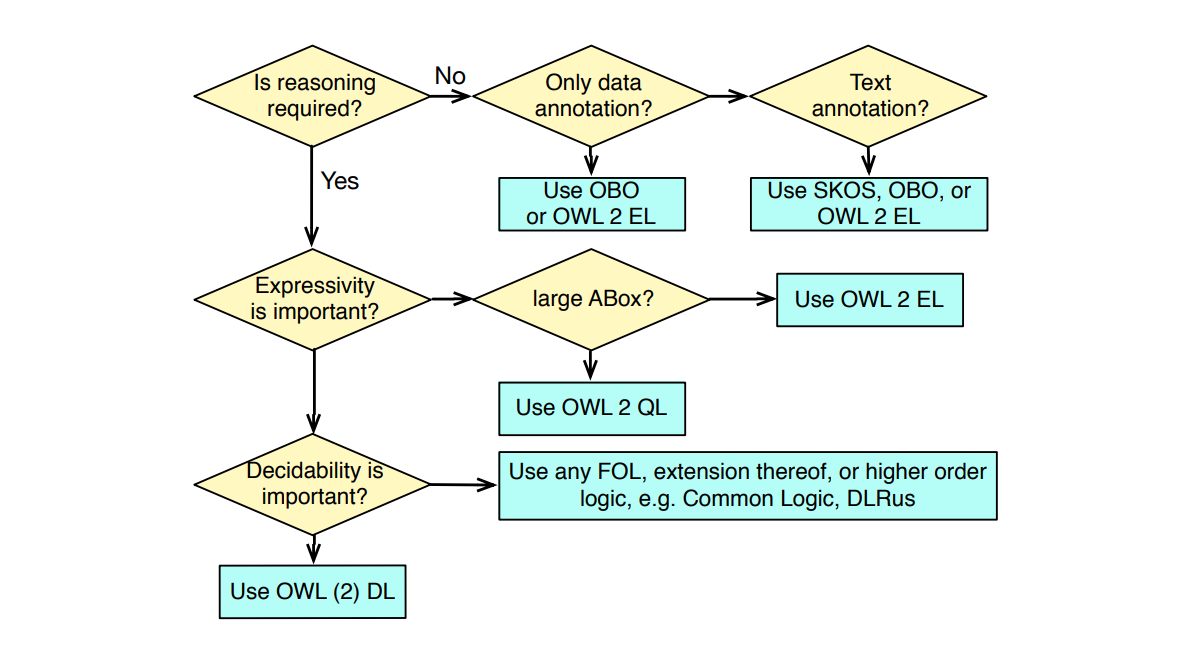
\includegraphics[scale=0.55]{lang.png}
	\caption{Diagram pomagający przy wyborze języka (źródło: \cite{lang})}
\end{figure}


\subsection{Metodyki}

Prawie w każdej dziedzinie życia jest wiele rozwiązań tego samego problemu, tak samo w ontologiach jest wiele różnych metodyk, jedną z nich jest np IDEF5 z 1989 roku \cite{repr_inf}. Zakłada ona przedstawienie pewnych informacji takich jak obiekty, relacje między nimi, oraz wartości w sposób uporządkowany składający się z elementów takich jak \cite{wikipediaIDEF5}:
\begin{itemize}
	\item język graficzny
	\item język tekstowy
	\item metoda w jaki sposób przechwytywać ontologie
\end{itemize}

W każdej z wcześniejszych metodologii można znaleźć wiele metod, które są dopełnieniem procesu tworzenia ontologii. Osoba tworząca ontologie często musi zadać sobie pytanie w jaki sposób pokazywać ją użytkownikowi - może to być za pomocą diagramów, ale również w sposób tekstowy. W Metodykach najczęściej mamy podejścia filozoficzne, logiczne lub mieszane. 

OntoClean pomaga w znajdywaniu błędów w taksonomii, czyli kategoryzacji elementów. Wykorzystując pojęcia z filozofii takie jak:
\begin{itemize}
	\item sztywność (zapis: +R dla sztywności, oraz -R dla braku sztywności)
	\item tożsamość (zapis: +I dla tożsamości, oraz -I dla braku tożsamości)
	\item jedność (zapis: +U dla jedności, oraz -U dla braku jedności),
\end{itemize}
oraz dzięki dopasowanym im elementom składni pomaga w tworzeniu łatwiejszych do zrozumienia ontologii \cite{fil_1}\cite{fil_2}. Klasa człowiek jest sztywna, ponieważ przez całe życie człowiek jest człowiekiem, natomiast klasa student nie jest sztywna, ponieważ studentem jest się przez jakiś okres czasu w życiu. Aby można było odróżnić klasy od siebie ważna jest ich tożsamość. Jeśli występuje niejednoznaczność w odróżnieniu od siebie instancji, należy przyjąć, że są one różne. W OntoClean występują sortale, tzn takie klasy, których byty są identyfikowane jako ten sam obiekt. Klasa, która jest sortalem wymusza, na jej podklasach również bycie sortalami. Jednościami są indywidualności, których wszystkie części są połączone tylko ze sobą, przez wyodrębnioną relację \cite{OntoClean}.

Przez to, że przy tworzeniu ontologii można popełnić wiele błędów, zostały one zapisane w postaci tzw antywzorców, lub katalogu pułapek \cite{oops}, z których część można wykryć automatycznie za pomocą OntOlogy Pitfall Scannera!(OOPS!). Jednym z takich błędów jest np. tworzenie synonimów jako klas, lub łączenie różnych pojęć w tej samej klasie.\cite{C.MariaKeet.2020}

\begin{figure}[h]
	\centering
	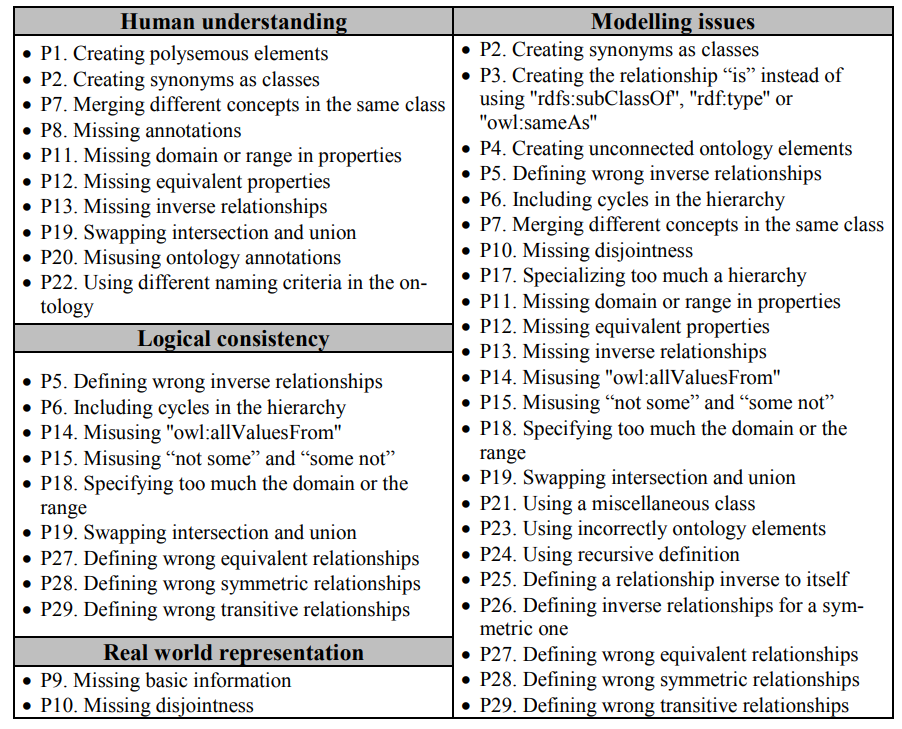
\includegraphics[scale=0.55]{tab_oops.png}
	\caption{Tabela pułapek (źródło: \cite{oops})}
\end{figure}

\chapter{ODE}

\section{Czym jest ODE}

ODE jest środowiskiem programistycznym, który umożliwia oraz pomaga tworzyć własne ontologie. Każdy programista tworzący oprogramowania lub ontologie, wie jak ważne jest odpowiednio przystosowane do tego środowisko, zapewniające odpowiednią ilość funkcji, intuicyjny interfejs, czasami obsługę dodatków, które wprowadzają usprawnienia, czy zmieniają motyw, dzięki czemu osoba korzystająca z niego może czuć się bardziej komfortowo. Szerokie upodobania użytkowników, powodują powstawanie wielu różnych edytorów ontologii, dzięki czemu każdy jest w stanie dopasować je pod własne preferencje wizualne, czy pod określoną funkcjonalność. Edytory te mogę różnić się chociażby językami jakie wspierają.
Jednymi z najbardziej znanych oraz mających często bardzo różną funkcjonalność środowisk są:
\begin{itemize}
	\item Protégé
	\item NeOn Toolkit
	\item SWOO.P
	\item TopBraid Composer
	\item Vitro
	\item Knoodl
	\item OWLGrEd (który jest edytorem graficznym)
\end{itemize}

\section{Zastosowania oraz działanie ODE}

W tej pracy działanie edytorów ontologii jest przedstawione na podstawie edytora Protégé, który jest jednym z najbardziej znanych, i najczęściej używanych programów do tworzenia i zarządzania ontologiami. Baza zarejestrowanych użytkowników strony oprogramowania, zawiera 366 084 kont \cite{protegecli}, mimo iż nie jest to wymagane do pobrania programu(wymagane jest do wersji webowej). Jego popularność może być zasługą tego, że jest otwarto-źródłowy oraz darmowy. Został stworzony w centrum badań informatyki biomedycznej w szkole medycznej Uniwersytetu Stanforda w Kalifornii \cite{protegeabout}.

Na samej górze interfejsu użytkownika (Rys. 2.1) znajduje się proste menu, w którym można znaleźć takie opcje jak: otworzenie ontologii z pliku w formatach: .pont, .pins, .xml, .owl, .rdf; możliwe jest dodawanie nowych zakładek takich jak widok klas czy OWL Viz, który pokazuje w sposób graficzny klasy i relacje między nimi.
\begin{figure}[h]
	\centering
	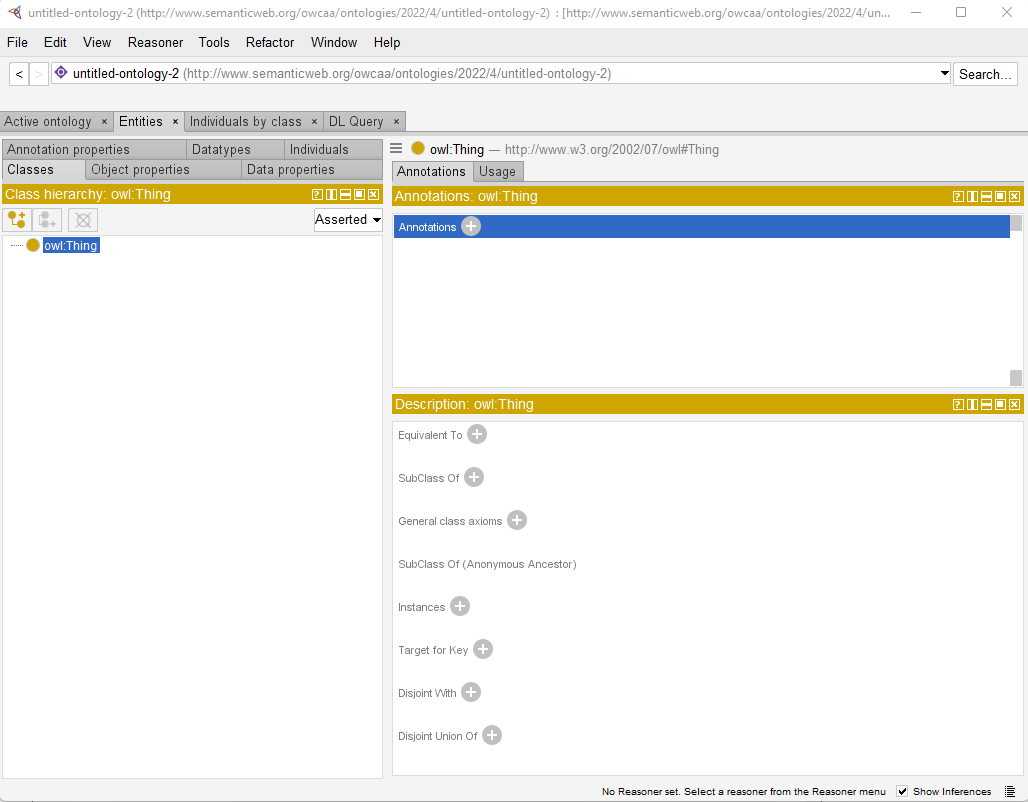
\includegraphics[scale=0.55]{Protege.png}
	\caption{Protege}
\end{figure}
W widoku klas można dodawać nowe klasy, oraz konkretnym z nich dodawać opisy, którymi mogą być:
\begin{itemize}
	\item równoważność do innej klasy
	\item jest podklasą
%	\item aksjomat klasy ogólnej
	\item nad klasy
	\item instancje (obiekty)
%	\item cel dla klucza
	\item rozłączność z
%	\item rozłączenie unii
\end{itemize}

Kolejną ważną zakładką jest właściwości obiektu w której można tworzyć relacje między obiektami. Każda taka relacja może w swoim opisie zawierać np.
\begin{itemize}
	\item równoważność
	\item jest pod własnością
	\item odwrotność
	\item domenę %nie rozumiem
	\item zakres
\end{itemize}

W zakładce właściwości danych można tworzyć dane konkretnych typów, oraz nadawać im właściwości takie jak:
\begin{itemize}
	\item równoważność
	\item jest pod własnością
	\item domenę 
	\item zakres
\end{itemize}
W karcie indywidualność jest możliwość tworzenia instancji konkretnych klas, dodania typów, równoważności, odmienności instancji do innej, oraz wcześniej utworzonych właściwości danych/obiektów.
OWLViz pozwala nam oglądać hierarchię klas w postaci grafów, gdzie można za pomocą przycisków sterować tym, które klasy i ich podklasy mają być pokazywane. Podobnie działa OntoGraf.

Jest to tylko część z funkcjonalności jakie posiada Protege. Jest to bardzo rozbudowane środowisko do tworzenia i zarządzania ontologiami, co ma swoje zalety, jak i wady które zostały opisane w następnych rozdziałach.

\section{Problemy istniejących ODE oraz potencjał rynkowy}
Potencjał rynkowy jest to "szacowanie maksymalnej, możliwej do osiągnięcia przez wszystkie firmy na danym rynku wielkości sprzedaży" \cite{Strategie}. Upraszczając definicję można wywnioskować, że produkt który jest tworzony musi być lepszy pod jakimś względem od aktualnie dostępnych, żeby móc trafić w mniej zagospodarowany przez firmy teren, które np. są dłużej na rynku. Gdy obiekt zbytu trafia do wielu konsumentów, łatwiej jest zbadać ich potrzeby, oraz oczekiwania. Ciężko określić potencjał rynkowy programu do tworzenia i zarządzania ontologiami, ze względu na małą ilość osób, które kiedykolwiek miało styczność z takimi edytorami.
\section{Ankieta}
W celu lepszego zrozumienia rynku, oraz potrzeb konsumentów z polski, została przeprowadzona ankieta w formularzach docs od google.
Nacisk położono na jak najmniejszą ilość punktów, na to żeby były krótkie, i aby w otwartych z nich dać ankietowanym przykłady odpowiedzi. Opracowane pytania zostały ułożone w sposób logiczny, od najbardziej ogólnych do bardziej szczegółowych:
\begin{itemize}
	\item Czy wiesz czym są ontologie?
	\item Czy słyszałeś kiedyś o edytorach ontologii?
	\item Czy korzystałeś kiedykolwiek z edytora ontologii?
	\item Jeśli tak to jakie problemy napotkałeś (nieintuicyjny interfejs, brak lub zbyt wiele funkcji itp)
	\item Co nie podoba Ci się w oprogramowaniu ze zdjęcia (zdjęcie pochodzi z edytora Protege)
\end{itemize}
Wyniki, mają za zadanie wskazać jak duże jest zainteresowanie ontologiami, wśród ludzi młodych, jakie problemy napotykają w ontologiach, oraz ich spostrzeżenia na temat protege.


\subsection{Analiza wyników ankiety}
 Analizując odpowiedzi z ankiety, w której udział wzięło 50 osób, wynika że ponad połowa nie miała styczności z takimi programami, i nie posiadają wiedzy czym są ontologie (Rys. 2.2). Wnioskując po odpowiedziach można wysnuć tezę, że taki projekt nie znajdzie bardzo szerokiego grona odbiorców. 
 
 Ankietowani, którzy korzystali z edytorów ontologii, lub którym interfejs Protege nie spodobał się, wymienili problemy takie jak:
\begin{itemize}
	\item przestarzały interfejs
	\item brak trybu ciemnego
	\item brak przechowywania plików w chmurze
	\item brak języka polskiego
	\item zbyt wiele funkcji, przez co problematyczne jest wdrożenie się do środowiska
	\item brak wprowadzenia(poradnika w postaci wyskakujących okien przedstawiających interfejs, przy pierwszym korzystaniu z oprogramowania)
\end{itemize}
Aby zachęcić użytkowników innych programów do zmiany swoich edytorów na rzecz tego zaprojektowanego w tej pracy, powinien on być pozbawiony większości problemów wymienionych przez ankietowanych.
\begin{figure}[h]
	\centering
	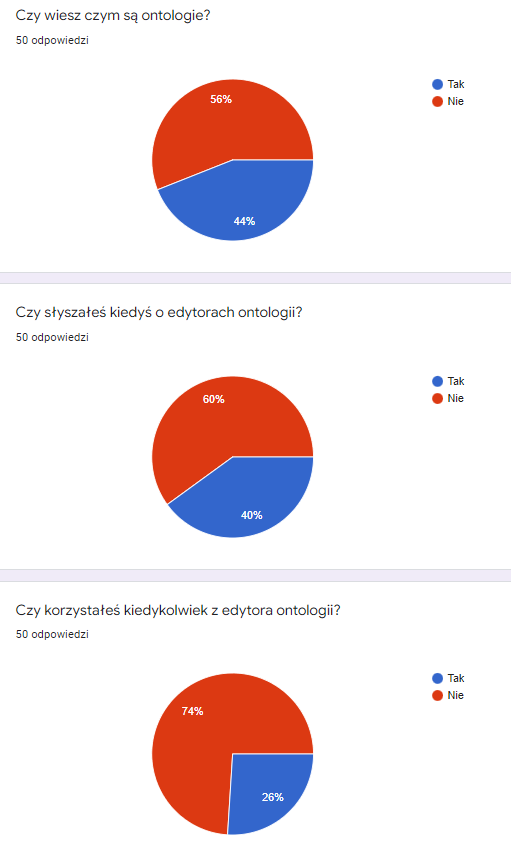
\includegraphics[scale=0.80]{wyn_ank.png}
	\caption{Wyniki przeprowadzonej ankiety}
\end{figure}

\chapter{Zebranie wymagań oraz projekt aplikacji}

\section{FURPS}
FURPS  (functionality, usability, reliability, performance, supportability - funkcjonalność, użyteczność, niezawodność, wydajność, wsparcie) \cite{furps} jest to model pomagający zebrać jak największą ilość wymagań jakie projekt powinien spełniać. Został on wymyślony przez Roberta Gready'ego który stworzył listę 5 głównych zagadnień, których przynajmniej w teorii opracowanie powinno pomóc pozbyć się większości nieścisłości i problemów jakie użytkownicy, oraz klienci dla których projektuje się aplikacje mogą napotkać w przyszłości.

\begin{figure}[h]
	\centering
	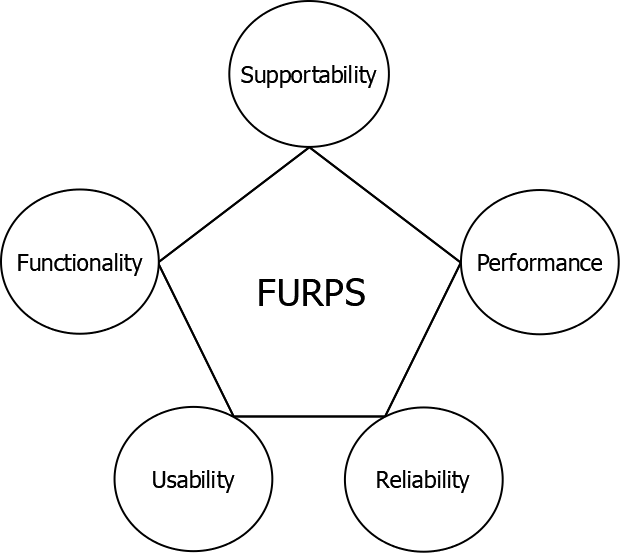
\includegraphics[scale=0.35]{Diagram2.png}
	\caption{model FURPS}
\end{figure}

Każdy z tych 5 punktów można rozwinąć o kolejne podpunkty (Tab. 3.1). 

	\begin{table}[!h]
		\resizebox{16cm}{!}{
		\centering
		\begin{threeparttable}
			\begin{tabular}{@{} l S[table-format=3.0] l S[table-format=4.0] cc @{}} 
				\toprule
				{Funkcjonalność} & {Używalność} & {Wydajność} & {Niezawodność} & {Wsparcie}\\
				\midrule
				Wymagania klienta & Spójność & {Przepustowość} & {Dokładność} & {Adaptowalność} \\
				Zapisywanie logów & {Estetyka} & Responsywność & Awaryjność & {Kompatybilność} \\ 
				Połączenia & {Ergonomia} & Skalowalność & Samonaprawa & Szybkość napraw \\
				Możliwość rozbudowy & {Dostępność} &  &  &\\
				Licencjonowanie & Lokalizacja językowa &  &  &  \\
				 & {Wsparcie użytkownika} &  &  &  \\
				\bottomrule
			\end{tabular}
			\caption{Rozwinięcie pkt. z FURPS (źródło: \cite{furps})}
		\end{threeparttable}}
	\end{table}

\section{Projekt aplikacji}
\subsection{Funkcjonalność}
Projektując ODE główny nacisk został postawiony na wybranie najbardziej potrzebnych funkcji niezbędnych do tworzenia ontologii i przedstawienie ich w prostej formie, żeby nowy użytkownik czuł się pewnie poruszając się po interfejsie, i żeby nie przytłaczała go ilość funkcji.

Aktorami są użytkownicy, którzy nie mają wielkiej wiedzy z zakresu ontologii, oraz osoby, którzy nie mają wysokich wymagań w stosunku do ilości funkcji jakich potrzebują do tworzenia ontologii.

Kluczowymi opcjami jakie posiada praktycznie każde środowisko programistyczne, i które również to będzie posiadało są:
\begin{itemize}
	\item otworzenie pliku (z serwera lub komputera)
	\item utworzenie pliku
	\item zapisanie (na serwerze lub komputerze)
	\item usunięcie pliku
	\item zmiana nazwy pliku
\end{itemize}
Aby umożliwić użytkownikowi zapisywanie swoich ontologii na serwerze, każdy klient będzie obowiązkowo potrzebował założyć własne konto w ODE, oraz logować się na stronie w celu weryfikacji tożsamości, i przydzielenia dostępu do odpowiednich plików. Przy rejestracji będzie wymagane podanie:
\begin{itemize}
	\item e-maila 
	\item hasła
	\item powtórnie hasła
\end{itemize}
Przy logowaniu natomiast wystarczy:
\begin{itemize}
	\item e-mail jako login
	\item hasło
\end{itemize}
Jeśli użytkownik zapomniałby swojego hasła, będzie możliwość zmiany, po podaniu maila, zostanie wysłany link resetujący hasło. Przy pierwszym logowaniu, użytkownik będzie przeprowadzony przez program dzięki wyskakującym okienkom opisującym podstawową funkcjonalność.

Kolejnymi ważnym funkcjami, które są już związane głównie z ontologiami są:
\begin{itemize}
	\item w zarządzaniu klasami, własnościami obiektów, oraz własnościami danych:
	\begin{itemize}
		\item dodanie podklasy/pod własności obiektu/pod własności danych
		\item dodanie równej klasy/własności obiektu/własności danych
		\item usunięcie samej klasy, lub wszystkich jej podklas razem z nią
	\end{itemize}
	\item w zarządzaniu indywidualnościami klas:
	\begin{itemize}
		\item dodanie indywidualności
		\item usunięcie indywidualności
	\end{itemize}
	Do każdej z klas można usunąć, lub dodać jako opis:
	\begin{itemize}
		\item równość klasy do innej
		\item nad klasy(super klasy)
		\item instancje
	\end{itemize}
	Do każdej z indywidualności można usunąć, lub dodać jako opis:
	\begin{itemize}
		\item typ (z jakiej klasy pochodzi)
		\item równość indywidualności do innej
		\item przypisanie właściwości danych
	\end{itemize}
	Do każdej własności obiektów można usunąć, lub dodać jako opis:
	\begin{itemize}
		\item równość własności do innej
		\item nazwy własności, których jest pod własnością
		\item własność, z którą jest odwrotna
		\item domenę
		\item zasięg
	\end{itemize}
	Do każdej własności danych można usunąć, lub dodać jako opis:
	\begin{itemize}
		\item równość własności do innej
		\item nazwy własności, których jest pod 3ewłasnością
		\item zasięg
		\item domenę
	\end{itemize}
\end{itemize}

\subsection{Używalność, wydajność, niezawodność i wsparcie} 
Zwracając uwagę na wyniki ankiety, które zostały opisana w rozdziale 2.4.1, ODE zostało zaprojektowane w stylu nowoczesnym, który objawia się między innymi tym, że elementy widoczne na ekranie są zaokrąglone, oraz posiadają lekkie cienie co dodaje wrażenia trójwymiarowości. Tryb ciemny, również jest czymś co klient może odebrać jako obcowanie z nowoczesnym oprogramowaniem. Z lokalizacji językowej jaka znajduje się na stronie jest język angielski jako domyślny, oraz polski. Dzięki temu, że kod został udostępniony publicznie na platformie github \cite{github} w ramach otwartej licencji, użytkownicy po przez wątki, które będą mogli poruszać, otrzymają informacje jak rozwiązać ich problemy, a bardziej ambitni z nich, będą mieli możliwość dodawania własnej funkcjonalności, która będzie mogła być w przyszłości(po weryfikacji) dodana do ODE. Ważne jest również to, aby do oprogramowania powstały automatyczne testy. Wiele osób uważa, że większość projektu , zajmują testy jednostkowe, które sprawdzają poprawność napisanego kodu. Aktualnie nie ma w projekcie uwzględnionej dostępności dla osób z niepełnosprawnościami, ani wersji mobilnej, która najprawdopodobniej w tego typu oprogramowaniu była by niemożliwa do stworzenia w sposób ergonomiczny. Strona powinna być kompatybilna z najnowszymi wersjami przeglądarek internetowych takich jak:
 \begin{itemize}
 	\item Google Crhome
 	\item Microsoft Edge
 	\item Safari
 	\item Mozilla Firefox
 	\item Opera
 \end{itemize}


Przez to, że grupa do, której kierowany jest produkt jest niewielka, obciążenie serwera również nie będzie duże. Można założyć, że miesięcznie na stronie pojawi się około 50 użytkowników z maksymalnie około 10 w jednym momencie. Każdy z nich powinien mieć własne miejsce do zapisu. Przykładowy plik ontologii o pizzach zajmuje około 130 KB miejsca na dysku \cite{pizza}. Przyjmując, że każdy użytkownik posiadałby średnio 3 takie pliki, potrzebne by było 6500 KB ($\sim$0,01 GB) miejsca na dane. Pliki aplikacji, oraz użytkowników będą znajdować się na jednym serwerze, który powinien mieć przynajmniej 0,5 GB miejsca na dane.


W możliwościach rozwoju należy uwzględnić zaprojektowanie motywu wysokiego kontrastu, funkcji czytaj, która zamieniała by treść strony na mowę, dodanie możliwości udostępniania swojej ontologii innym użytkownikom, oraz projekt wizualizacji ontologii za pomocą grafów. W kwestii poprawy bezpieczeństwa będzie wymagane zaprojektowanie uwierzytelniania wielopoziomowego. Gdyby, dysk zaczął się zapełniać, przy 80\% należy dokupić 50\% więcej miejsca.

\subsection{Klasy, oraz przypadki użycia}

Projekt zakłada 5 klas, którymi są (Rys. 3.2):
\begin{itemize}
	\item Ontology
	\item ClassMan
	\item InstanceMan
	\item ObjectPropertyMan
	\item DataPropertyMan
\end{itemize}
\begin{figure}[h]
	\centering
	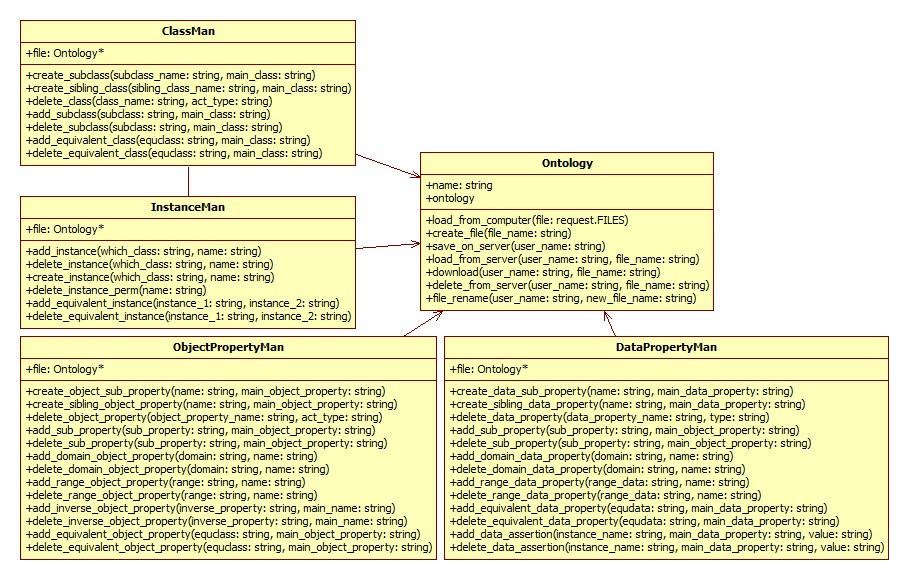
\includegraphics[scale=0.5]{klasy.jpg}
	\caption{Diagram klas}
\end{figure}
 Klasa Ontology zapewnia obsługę plików ontologii użytkownika, natomiast reszta pozwala na zarządzanie podzielonymi odpowiednio na klasy, instancje, właściwości obiektów i właściwości danych elementami ontologii.
 
   Stworzony diagram przypadków użycia (Rys. 3.3), przedstawia w sposób ogólny interakcje z aktorem, ramy systemu, oraz przypadki użycia. Użytkownik może stworzyć konto. Aktor, żeby zarządzać plikami ontologii będzie musiał się zalogować. Zarządzanie klasami, instancjami, właściwościami obiektów/danych rozszerza zarządzanie ontologiami, które rozszerza operowanie na plikach ontologii.
 
  \begin{figure}[h]
 	\centering
 	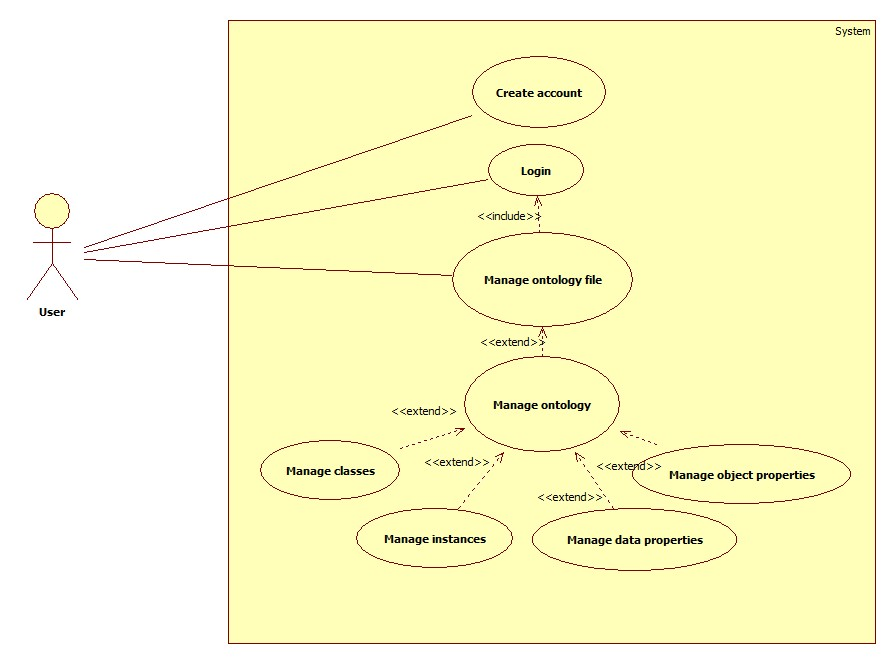
\includegraphics[scale=0.5]{UseCaseDiagram.jpg}
 	\caption{Diagram przypadków użycia}
 \end{figure}
 
  Większość zaproponowanych metod powinna być zrozumiała, natomiast należy rozróżnić metody delete$\_$instance oraz delete$\_$instance$\_$perm, pierwsza metoda usuwa instancje z opisu klasy, natomiast druga odpowiada za całkowite jej usunięcie.

 


Najbardziej rozbudowaną metodą jest ta, odpowiadająca usuwaniu klas, właściwości obiektów, oraz właściwości danych (Rys. 3.4). Zostaje jej przekazana nazwa usuwanego elementu, oraz typ(w jaki sposób usnąć). Gdy użytkownik usuwa jedną klasę(bez podklas), najpierw podłączone zostają jej podklasy do jej nad klasy, a następnie zostaje usunięta klasa, której nazwa została przekazana do metody. Kiedy użytkownik chce usunąć wszystkie podklasy, metoda przechodzi rekurencyjnie po podklasach przekazując je sobie, do momentu, aż nie będzie żadnych, i usuwa klasę, która była przekazana jako ostatnia. Następnie wraca do wcześniejszych, i usuwa je. Analogicznie działa to dla właściwości obiektów, oraz właściwości danych.

\begin{figure}[h]
	\centering
	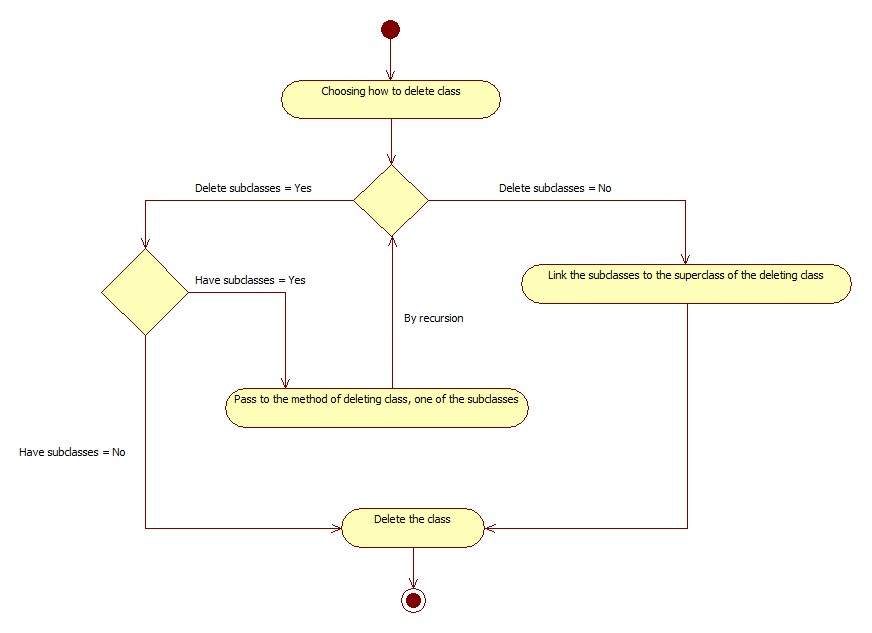
\includegraphics[scale=0.5]{ActivityClassDiagram.jpg}
	\caption{Diagram aktywności}
\end{figure}



\subsection{Interfejs}
Graficzny interfejs użytkownika(GUI) został zaprojektowany w sposób nowoczesny (Rys. 3.5). Przeważają w nim odcienie białego, pomarańczowego, różowego, oraz niebieskiego. Cienie dodają wrażenia trójwymiarowości. Na górze interfejsu znajdują się przyciski language, oraz change mode, które pozwolą odpowiednio na zmianę języka i włączenie trybu ciemnego(bądź wyłączenie). W centralnym punkcie znajduje się miejsce na wprowadzenie nazwy użytkownika, oraz hasła. Strona rejestracji różni się tylko częścią środkową (Rys. 3.6). Ciemny motyw zakłada zmianę barwy tła, z białej, na ciemnoszarą, dopasowanie koloru czcionki, żeby była czytelna, oraz zmianę wypełnień przycisków language na różowy, oraz przycisku register na ciemniejszy szary (Rys. 3.7).

Na stronie głównej (Rys. 3.8) w pasku nawigacyjnym  został dodany przycisk file w takim samym stylu jak language, powitanie użytkownika po jego nazwie, oraz wylogowanie. Niżej znajdują się przyciski pozwalające na zmianę aktualnie przeglądanych elementów ontologii.
W przestrzeni po lewej stronie, jest wyświetlana hierarchia odpowiadająca aktualnie wybranej opcji np. klas, z rozwijanymi listami tych klas, oraz możliwością dodawania podklas, klas bliźniaczych i usuwania ich. Po prawej stronie opis aktualnie wybranej klasy z możliwością usuwania oraz dodawania kolejnych elementów do opisu.



\begin{figure}[h]
	\centering
	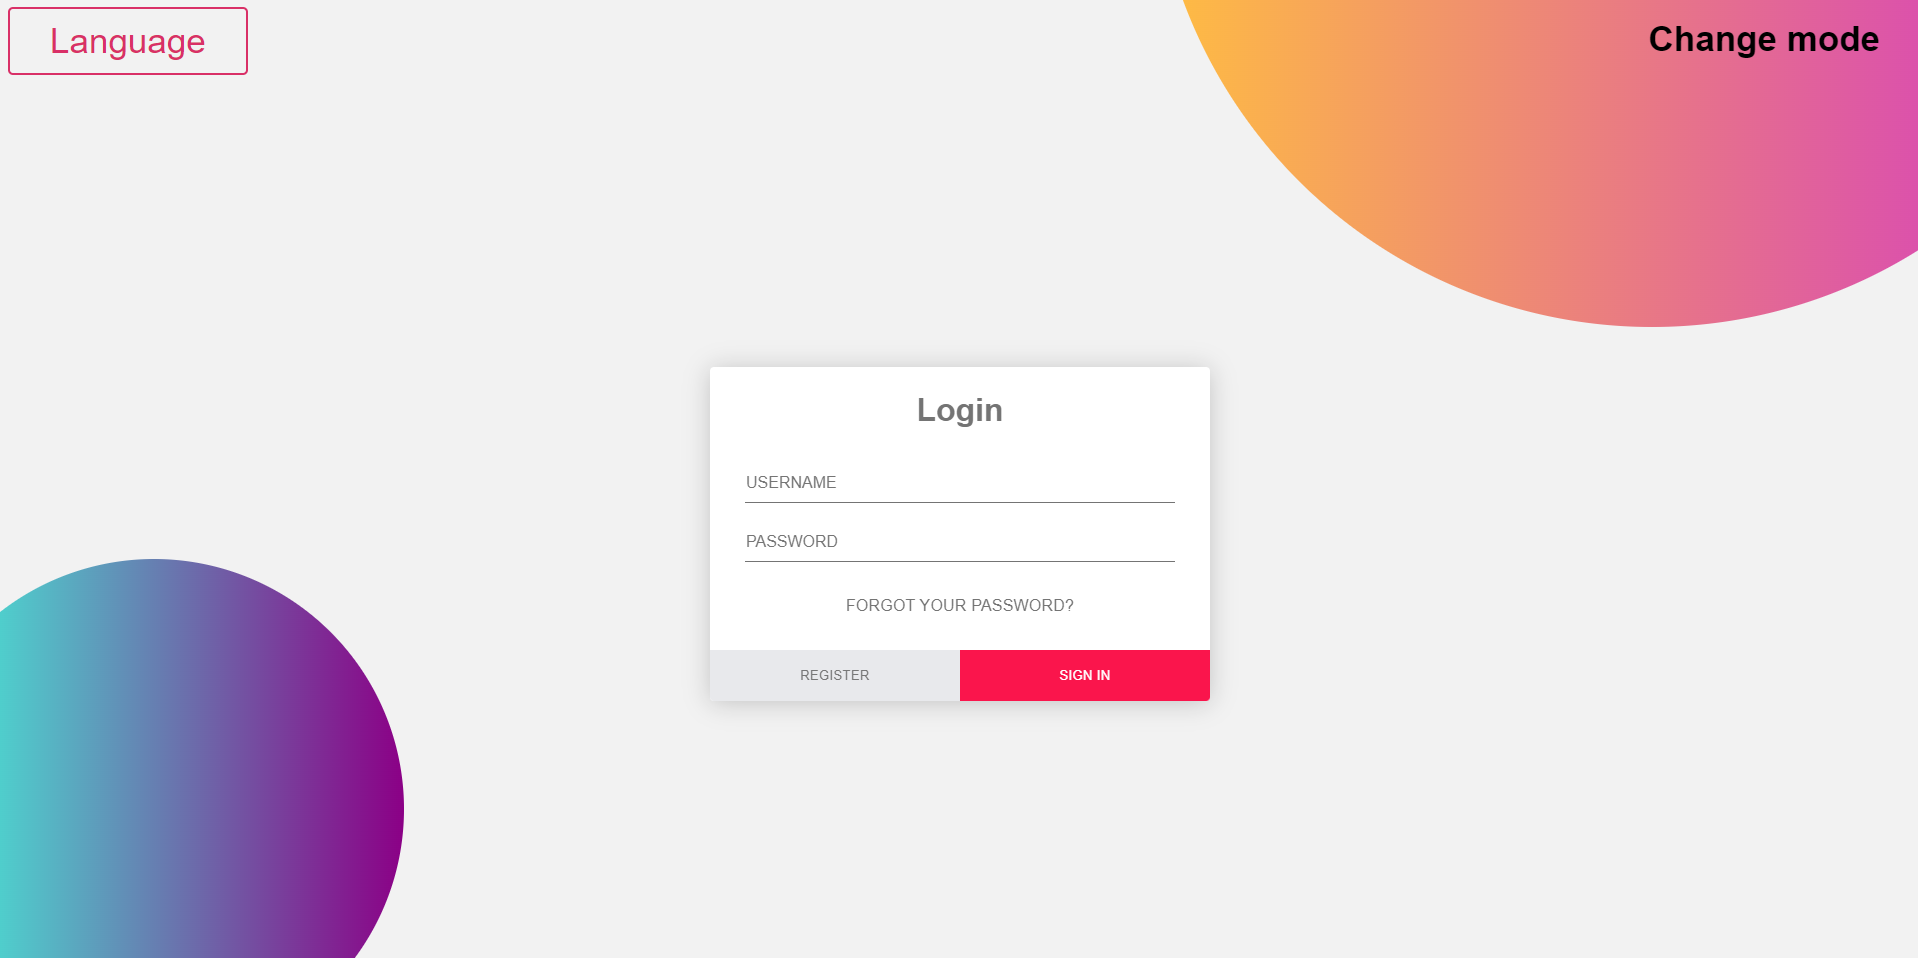
\includegraphics[scale=0.31]{login_page.png}
	\caption{Strona logowania}
\end{figure}

\begin{figure}[h]
	\centering
	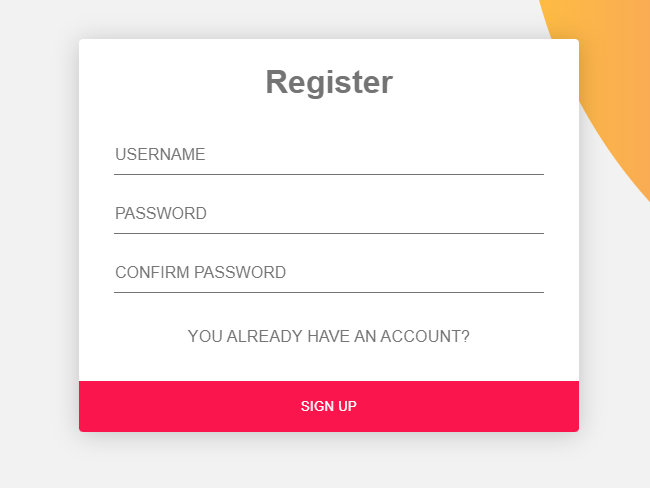
\includegraphics[scale=0.31]{register.png}
	\caption{Punkt centralny strony logowania}
\end{figure}

\begin{figure}[h]
	\centering
	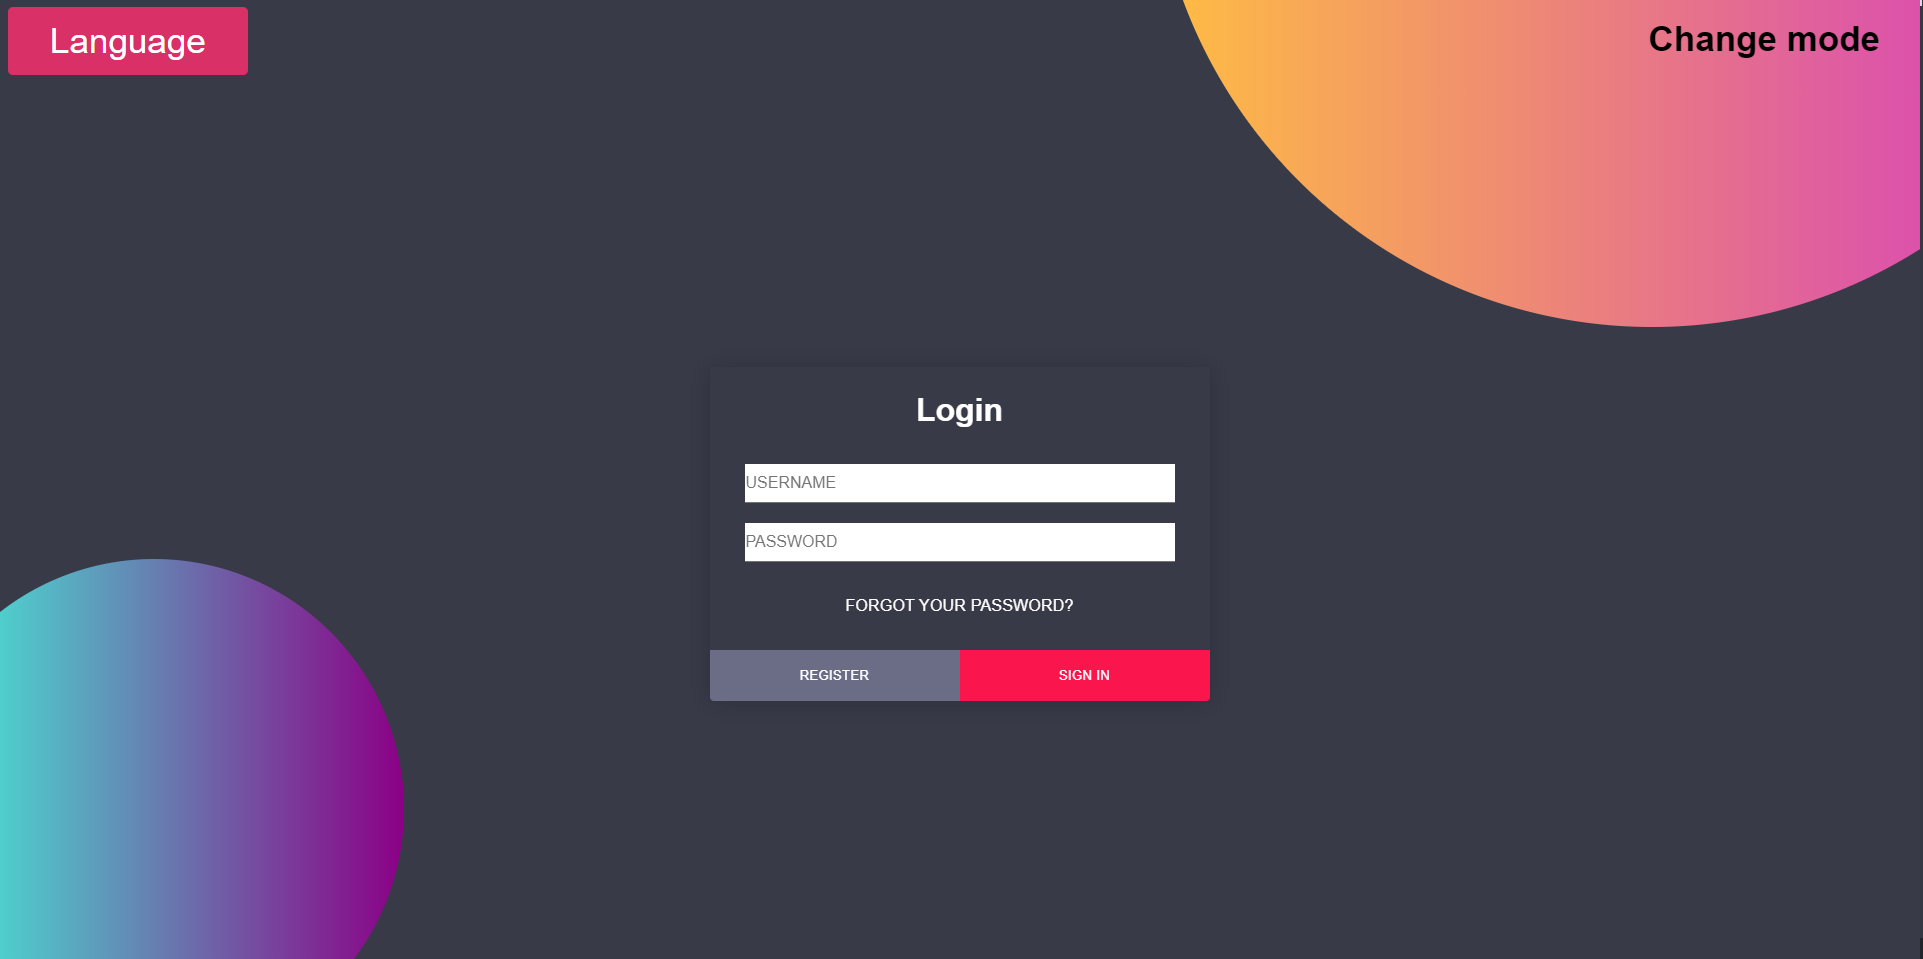
\includegraphics[scale=0.31]{dark_en.png}
	\caption{Strona logowania po angielsku i w trybie ciemnym}
\end{figure}

\begin{figure}[h]
	\centering
	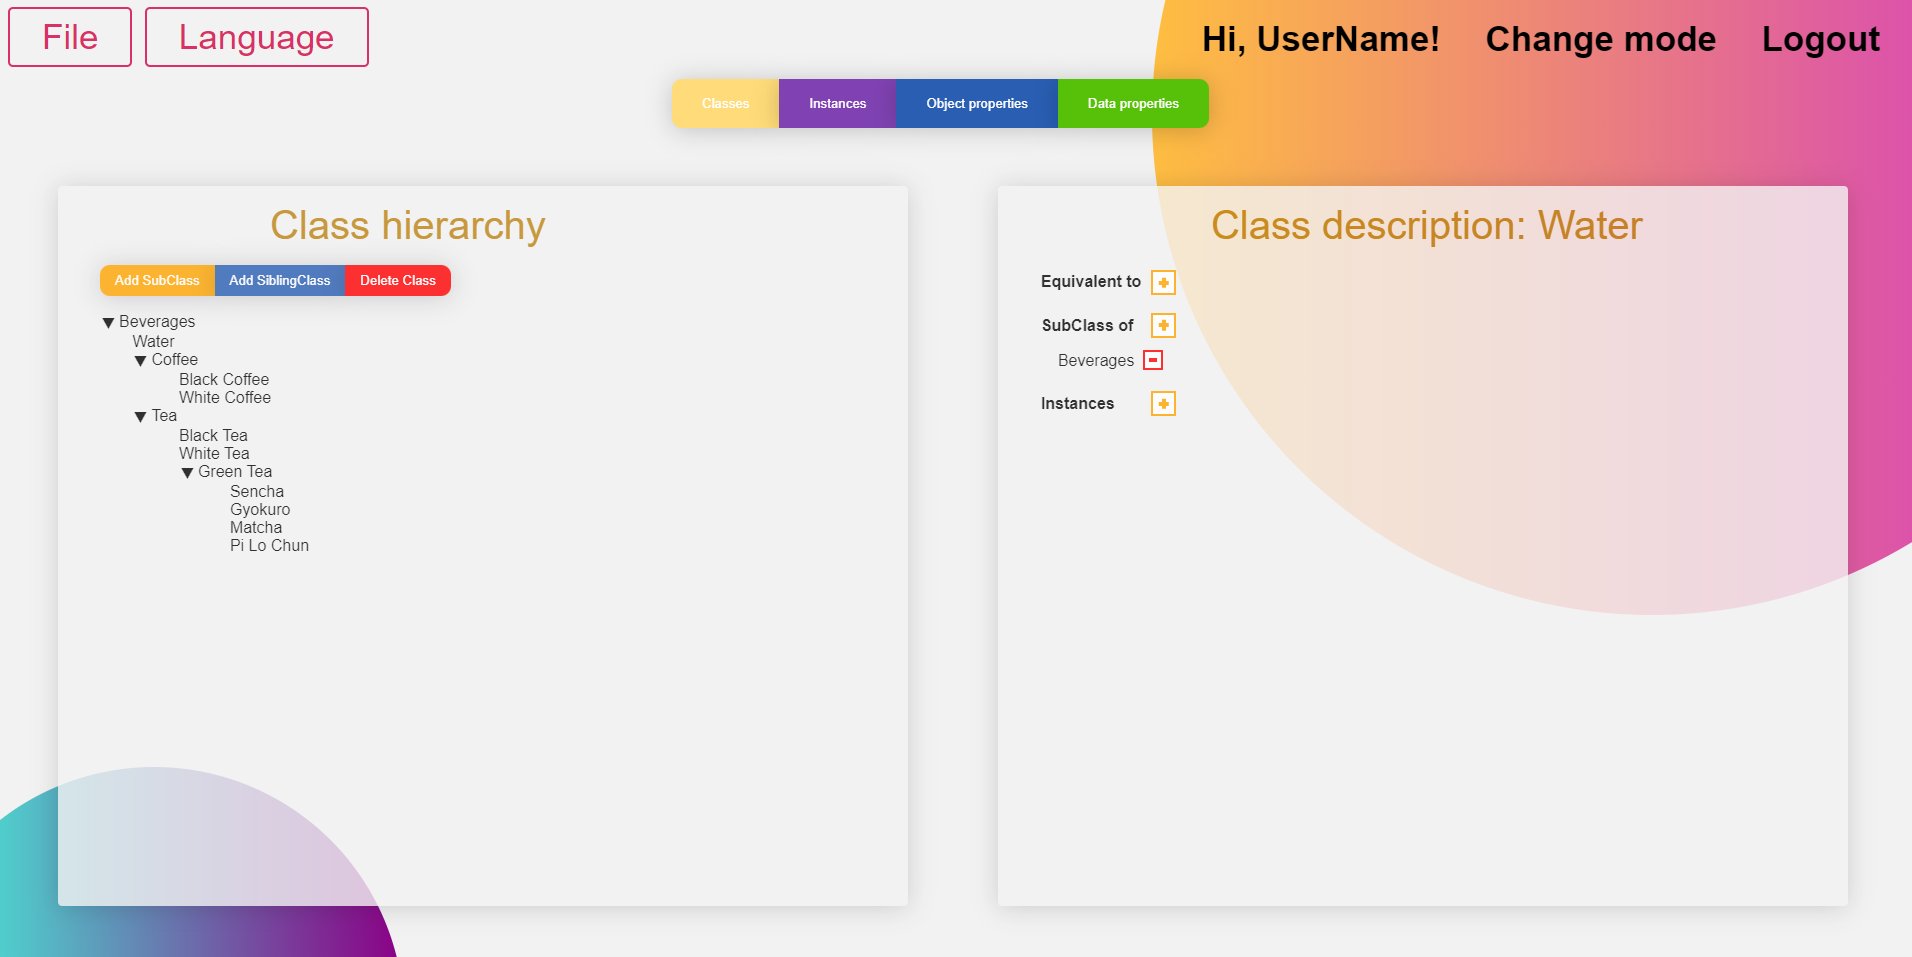
\includegraphics[scale=0.31]{main_page.png}
	\caption{Strona domowa}
\end{figure}

\chapter{Implementacja oraz przedstawienie wersji demonstracyjnej}
\section{Klasy}
Klasy zostały wykonane w oparciu o projekt z diagramu klas (Rys. 3.2),przy użyciu języka python3 \cite{python} i biblioteki Owlready2 \cite{owlready2}. W pliku file.py znajduje się klasa Ontology, której obiekty posiadają swoją nazwę i ontologie.
\begin{lstlisting}[language=Python, basicstyle=\small, breaklines=true, caption={Przykładowe metody klasy Ontology},  label={lst:class}]
	class Ontology:
		def __init__(self, file_name, ontology):
			self.name = file_name
			self.ontology = ontology
		
		def save_on_server(self, user_name):
			file_path = os.path.join(os.path.abspath(os.getcwd()), "data", user_name, "")
			if os.path.exists(os.path.dirname(file_path + self.name)):
				return HttpResponse(status=409)
		
			if not os.path.exists(os.path.dirname(file_path)):
				try:
					os.makedirs(os.path.dirname(file_path))
				except OSError as exc:
					if exc.errno != errno.EEXIST:
						raise
			self.ontology.save(os.path.join(file_path, self.name), format="rdfxml")
		
		def load_from_server(self, user_name, file_name):
			self.name = file_name
			file_path = os.path.join(os.path.abspath(os.getcwd()), "data", user_name, file_name)
			self.ontology = get_ontology(file_path).load()
		
		def file_rename(self, user_name, new_file_name):
			file_path_old = os.path.join(os.path.abspath(os.getcwd()), "data", user_name, self.name)
			file_path_new = os.path.join(os.path.abspath(os.getcwd()), "data", user_name, new_file_name)
			if not os.path.exists(os.path.dirname(file_path_old)):
				self.name = new_file_name
			else:
				os.rename(file_path_old, file_path_new)
\end{lstlisting}

W pliku ontology.py znajdują się wszystkie inne klasy, które zostały zaprojektowane i są potrzebne do zarządzania ontologiami. Każda z nich posiada obiekt klasy Ontology. Oparte są one na dynamicznym tworzeniu nowych klas. W implementacji brakuje usuwania wszystkich podklas, oraz pod własności obiektów/danych.

\begin{lstlisting}[language=Python, basicstyle=\small, breaklines=true, caption={Przykładowe metody klasy ClassMan},  label={lst:class}]
	class ClassMan:
		def __init__(self, file: Ontology):
			self.file = file
		
		def create_subclass(self, subclass_name, main_class):
			with self.file.ontology:
				if main_class == "Thing":
					new_class = types.new_class(subclass_name, (eval(main_class),))
				else:
					new_class = types.new_class(subclass_name, (self.file.ontology[main_class],))
		
		def create_sibling_class(self, sibling_class_name, main_class):
			with self.file.ontology:
				new_class = types.new_class(sibling_class_name, (list(self.file.ontology[main_class].is_a)[0],))
				
\end{lstlisting}

\section{Wersja demonstracyjna}
Do stworzenia wersji demonstracyjnej nowoczesnego ODE dla nowych użytkowników został użyty framework django \cite{dj}, który jest wykorzystywany do tworzenia stron internetowych (część back-endowa) w języku python3. Strony zostały napisane w języku znaczników jakim jest HTML, kaskadowych arkuszy stylów (CSS), oraz skryptów napisanych w JavaScripcie. Wersja testowa pokazuje interfejs, oraz system autoryzacji, który jest częścią django - posiada własny plik bazy danych sqllite, oraz metody do logowania, rejestracji, wylogowania i sprawdzania, czy użytkownik jest zalogowany. Aktualna implementacja pozwala na skorzystanie z 5 rozwinięć linków.

\begin{lstlisting}[language=Python, basicstyle=\small, breaklines=true, caption={Paterny URL},  label={lst:class}]
	urlpatterns = [
		path('login/' ,views.loginPage, name="login"),
		path('logout/' ,views.logoutUser, name="logout"),
		path('register/' ,views.registerPage, name="register"),
		path('', views.home, name="home"),
		path('login_pl/' ,views.loginPagePl, name="login_pl"),
	]
\end{lstlisting}
Pierwszą stroną jaka pokazuje się po uruchomieniu serwera developerskiego jest logowanie (Rys. 3.5), użytkownik jest w stanie zmienić język z angielskiego na polski(i z polskiego na angielski). Zmiana aktualnie działa tylko na stronie logowania. Po naciśnięciu przycisku rejestracji okno login zamienia się na okno z rejestracją. Funkcja generująca widok logowania, w polu kontekstowym, wysyła wiadomość jak ma być renderowana strona(logowanie lub rejestracja), a następnie dzięki warunkowi if w pliku login.html, wyświetla odpowiedni element na stronie.

\begin{lstlisting}[language=html, basicstyle=\small, breaklines=true, caption={Przykłaad okna rejestracji w htmlu},  label={lst:class}]
	
	.
	.
	.
	
	
	<div class="circlebig"></div>
	<div class="circlesmall"></div>
	<div class="login">
		<form method="POST" action="">
			
			<h1>Register</h1>
			<div class="content">
				<div class="input">
					{{form.username}}
				</div>
				<div class="input">
					{{form.password1}}
				</div>
				<div class="input">
					{{form.password2}}
				</div>
				<a href="" class="link">You already have an account?</a>
			</div>
			<div class="action">
				<div class="register">
					<button>Sign up</button>
				</div>
			</div>
		</form>
		
		<ul class="messages">
			
			<li>{{ message }}</li>
			
		</ul>
		
	</div>
\end{lstlisting}

Po zalogowaniu użytkownik zostaje przekierowany na widok domowy (Rys. 3.8). Na tej stronie jedyną funkcjonalnością jest możliwość wylogowania, która przekierowuje na widok logowania.

\begin{lstlisting}[language=Python, basicstyle=\small, breaklines=true, caption={Przykłaad funkcji wylogowania},  label={lst:class}]
	def logoutUser(request):
		logout(request)
		return redirect('login')
\end{lstlisting}

\chapter*{Zakończenie}
\addcontentsline{toc}{chapter}{Zakończenie}
W pracy zostały opisane języki, przy użyciu których tworzy się ontologie, ich historia, metodologie podzielone na mikro, oraz makro, metodyki takie jak np. OntoClean, a także działanie edytora Protege.
Dzięki ankiecie, która trafiła do wielu osób(50), można było wyciągnąć wnioski, które pomogły w lepszym zrozumieniu potrzeb klienta. Następnie zostały zebrane wymagania, możliwości rozwoju, wstępnie oszacowany ruch, wraz z ilością danych jakie są wymagane na pliki. Został stworzony diagram klas, ogólny diagram przypadków użycia, oraz diagram aktywności. Wykonany został projekt nowoczesnego gui, oraz implementacja klas, wraz ze stworzeniem wersji demonstracyjnej interfejsu, przy użyciu django.

Stworzenie oprogramowania, które trafia w gusta każdego klienta jest niemożliwe. Zawsze trzeba decydować się na różnego typu rozwiązania, oraz ustępstwa, dzięki czemu jest duża różnorodność na rynku, i każdy użytkownik jest w stanie znaleźć coś dla siebie. Projekt nowoczesnego ODE dla początkujących na pewno jest w stanie trafić w pewną niszę na rynku, gdzie ludzie oczekują ciągłego dostępu do swoich ontologii, i zwracają uwagę na wygląd oprogramowania, natomiast nie potrzebują wielu zbędnych funkcjonalności, których zapewne nigdy nie użyją. Demo, które zostało zaprezentowane potwierdziło użyteczność, oraz przydatność funkcji takich jak np. zmiana języka.

\listoftables{} % jeśli są tabele
\addcontentsline{toc}{chapter}{Spis tabel}

\listoffigures{} % jeśli są tabele
\addcontentsline{toc}{chapter}{Spis rysunków}
\lstlistoflistings
\addcontentsline{toc}{chapter}{Spis listingów}

\addcontentsline{toc}{chapter}{Bibliografia}
\printbibliography[title=Bibliografia]

 %\bibitem{textbook}
 %Krzysztof Goczyła: Ontologie w systemach informatycznych. Warszawa: Akademicka Oficyna Wydawnicza EXIT, 2011, s. 26–30. ISBN 978-83-60434-88-8.
  %\bibitem{textbox} https://www.w3.org/OWL/


\end{document}
